\documentclass[conference]{IEEEtran}
\usepackage{graphicx}
\usepackage{amsmath}
\usepackage{booktabs}
\usepackage{times}
\usepackage{url}

\begin{document}

\title{A Reproducible Benchmark for Slice-Level Infection Burden Scoring
on COVID-19 CT}

\author{
\IEEEauthorblockN{Jingnan Jia\textsuperscript{1,*}, Lisi Wang\textsuperscript{1}}
\IEEEauthorblockA{\textsuperscript{1}School of Public Affairs, Zhejiang University, Hangzhou, China\\
\texttt{jiajingnan@zju.edu.cn} (corresponding), \texttt{0624f01@zju.edu.cn}}
}

\maketitle

\begin{abstract}
Most COVID-19 CT scoring studies treat axial slices as independent, identically
distributed samples and report a single aggregate error. Both habits are
misleading on public data: slices are clustered within a handful of scans, and a
pooled error hides whether a model actually \emph{ranks} burden correctly. We
release a small, reproducible benchmark that fixes both problems. Using the
public COVID-19-CT-Seg dataset (Ma et al., Zenodo 3757476, CC-BY 4.0; 20
volumes, 2240 slices from 20 cases, so the effective sample is $N{=}20$), we
regress the slice infection burden $y=N_{\mathrm{inf}}/(N_{\mathrm{lung}}+N_{\mathrm{inf}})$
from a 22-D feature set (16-bin lung HU histogram, texture, gradient, lung-area
and left/right ratios). We (i) publish a \emph{fixed} 4-fold \emph{by-case}
partition and the per-slice features, and (ii) report every metric with a
\emph{case-level} 95\% bootstrap confidence interval. Six model families---a
median floor, ridge, a 2-layer MLP, Random Forest, Histogram Gradient Boosting
and an MLP regressor---are compared with and without the two anatomical
features. The anatomy effect is never significant: dropping it is at worst
neutral and often marginally improves MAE. Notably, the linear ridge model does
\emph{not} beat the trivial median floor on MAE, whereas the nonlinear models
do. We release code, features, splits and results so the community can compare
against a common, uncertainty-aware baseline.
\end{abstract}

\begin{IEEEkeywords}
COVID-19 CT, infection burden, benchmark, slice-level regression, case-level
uncertainty, reproducible study
\end{IEEEkeywords}

\section{Introduction}
Quantifying COVID-19 lung involvement per slice is more informative than a global
percentage, but manual segmentation does not scale and a practical model must
learn from coarse, mask-derived labels. Two reporting habits undermine such
studies. First, slices from one scan are correlated, yet results are quoted as if
2240 slices were 2240 independent samples---inflating apparent certainty.
Second, a single MAE hides whether predictions rank burden correctly, which is
what clinicians actually use. We contribute a benchmark that corrects both: a
fixed by-case split, released features, and case-level bootstrap confidence
intervals, on the public COVID-19-CT-Seg data.

\section{Related Work}
Automated CT scoring of interstitial lung disease is surveyed by Barnes et
al.~\cite{barnes2023mlradiology} and shown for systemic-sclerosis ILD by
Chassagnon et al.~\cite{chassagnon2020dl}; Jia et al.~\cite{jia2024explainable}
obtain explainable scores from per-region expert labels. Weak supervision from CT
appears in Wang et al.~\cite{wang2019weakild} and Djahnine et
al.~\cite{djahnine2024weak}, and anatomy--pathology disentanglement in
Ganin et al.~\cite{ganin2016dann}, Saito et al.~\cite{saito2018mcd}, Xie et
al.~\cite{xie2022disentangle} and Berens et al.~\cite{berens2026shortcut}.
Clinically, COVID-19 involvement is summarised by ordinal severity scores (e.g.\
RSNA, RALE), but these are coarse and reader-dependent; continuous, mask-derived
burden is a natural continuous target, and the public masks make it computable at
scale. Our benchmark addresses exactly this target.
\textbf{Distinction from the dataset paper:} Ma et al.~\cite{ma2021covidseg}
release segmentation \emph{masks}; they do not define a burden-regression task,
a fixed split, or any uncertainty estimate. Our benchmark sits on top of that
release and provides exactly those.

\section{Method}
\subsection{Per-slice features}
For each axial slice with lung area $>5\%$ of the frame we extract a 16-bin HU
histogram over $[-1000,400]$ (normalised), mean/std/skewness of lung HU, mean
gradient magnitude, lung-area ratio, and left/right lung-area ratio---a 22-D
vector. The label is $y=N_{\mathrm{inf}}/(N_{\mathrm{lung}}+N_{\mathrm{inf}})
\in[0,1]$, derived directly from the masks. The denominator includes
$N_{\mathrm{inf}}$ so that $y$ is the fraction of the total lung-plus-infection
region occupied by infection and is bounded in $[0,1]$; it is a monotone
transform of the lung-only ratio, so ranking metrics do not depend on this choice.

\subsection{Models and the anatomy ablation}
Six families: a \textbf{Median} constant floor, \textbf{Ridge} ($\alpha{=}1$), a
\textbf{2-layer MLP} (32 tanh units, Adam, 300 epochs), \textbf{Random Forest},
\textbf{Histogram Gradient Boosting}, and \textbf{MLPRegressor} (all scikit-
learn, fixed seed). Each is run with \textbf{A} (all 22 features) and \textbf{B}
(the two anatomical features removed). B is the analogue of ``disentanglement by
withholding'' and isolates whether anatomy carries recoverable information.
Hyper-parameters follow simple, conventional defaults (ridge $\alpha{=}1$; MLP 32
tanh units, Adam, 300 epochs; Random Forest 300 trees; HistGradientBoosting and
MLPRegressor at scikit-learn defaults) so the comparison isolates the
feature-choice question, not tuning.

\subsection{Cross-validation and uncertainty}
We use 4-fold CV \emph{split by case} (no slice leakage). The effective sample is
20 cases. For every metric we report the point estimate over all held-out slices
together with a \emph{case-level} 95\% bootstrap CI: we resample the 20 cases
with replacement 1000 times, pool their slices, and take the 2.5/97.5
percentiles of MAE and Spearman. This interval reflects case-level variability,
not the illusory precision of 2240 correlated slices.

\begin{figure}[!t]
\centering
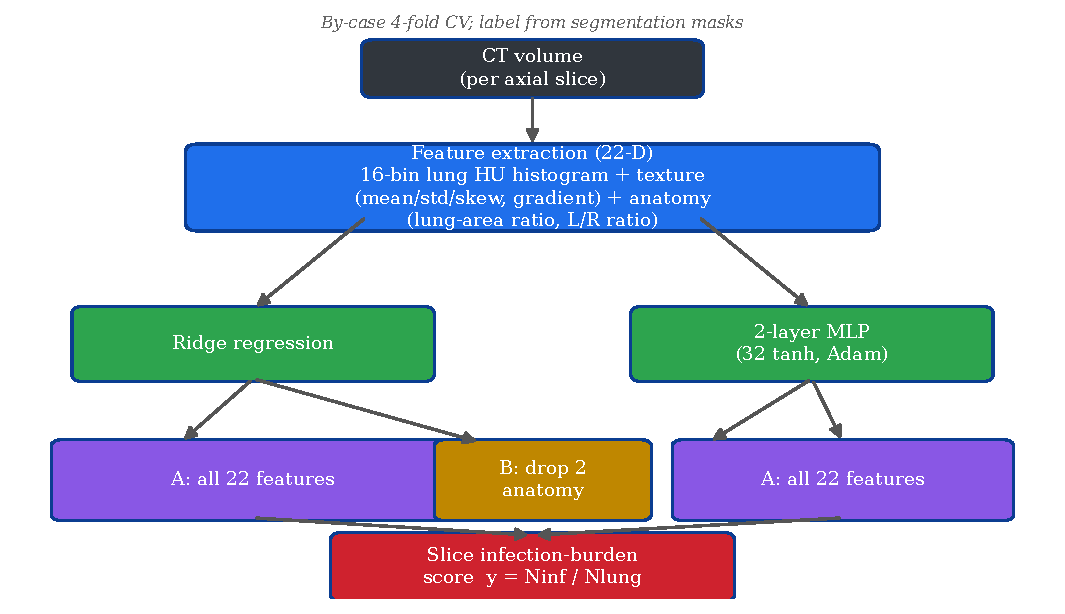
\includegraphics[width=\columnwidth]{figures/fig1_method.pdf}
\caption{Framework: each axial slice yields a 22-D vector; six regressors are
compared with (A) and without (B) the two anatomical features.}
\label{fig:meth}
\end{figure}

\section{Data and Benchmark Release}
We use COVID-19-CT-Seg (Ma et al.~\cite{ma2021covidseg}, Zenodo 3757476, CC-BY
4.0): 20 CT volumes with lung and infection masks. Keeping slices with lung area
$>5\%$ gives 2240 slices from 20 cases (28.2\% zero, median 0.034, max 0.615);
all labels are mask-derived, not reader scores. To make the study reproducible
we release: \texttt{data/features.csv} (one row per slice: case\_id, slice\_idx,
22 features, $y$); \texttt{data/splits.json} (the fixed seed-0 by-case 4-fold
partition); and \texttt{results/results\_real\_v2.json} with per-fold metrics,
point estimates and CIs (see \texttt{BENCHMARK.md}).

\section{Results}
\begin{table}[!t]
\centering
\caption{MAE and Spearman $\rho$ with the across-fold mean$\pm$std and a
case-level 95\% bootstrap CI (1000 resamples of the 20 cases). MAE lower is
better, $\rho$ higher is better. A/B = all 22 features / without the two anatomy
features; the last row is the image-based learned baseline (a trained-from-scratch
CNN underfit on 20 cases, so the downgraded Random-Conv-Features + Ridge is
reported). Median is a constant predictor, hence its $\rho$ is undefined (n/a). Values are across-fold means of per-fold estimates; the pooled out-of-fold point estimates quoted in the text can differ slightly (largest gap $\Delta\rho=0.084$).}
\label{tab:main}
\small
\begin{tabular}{llccc}
\toprule
Model & Feat & MAE (m$\pm$sd) & $\rho$ (m$\pm$sd) & 95\% CI (MAE; $\rho$) \\
\midrule
Median (floor) & --  & $0.0776\pm0.0223$ & n/a & $[0.048,0.108]$; n/a \\
Ridge & A & $0.0924\pm0.0082$ & $0.597\pm0.207$ & $[0.076,0.116]$; $[0.389,0.781]$ \\
Ridge & B & $0.0931\pm0.0088$ & $0.576\pm0.234$ & $[0.077,0.118]$; $[0.346,0.776]$ \\
MLP (2-layer) & A & $0.0658\pm0.0181$ & $0.367\pm0.182$ & $[0.047,0.083]$; $[0.186,0.617]$ \\
MLP (2-layer) & B & $0.0582\pm0.0139$ & $0.504\pm0.233$ & $[0.043,0.074]$; $[0.320,0.724]$ \\
Random Forest & A & $0.0685\pm0.0204$ & $0.407\pm0.148$ & $[0.048,0.087]$; $[0.304,0.614]$ \\
Random Forest & B & $0.0640\pm0.0156$ & $0.440\pm0.192$ & $[0.047,0.080]$; $[0.289,0.657]$ \\
HistGradBoost & A & $0.0690\pm0.0194$ & $0.383\pm0.189$ & $[0.050,0.087]$; $[0.251,0.594]$ \\
HistGradBoost & B & $0.0619\pm0.0141$ & $0.467\pm0.192$ & $[0.046,0.078]$; $[0.302,0.665]$ \\
MLPRegressor & A & $0.0749\pm0.0186$ & $0.494\pm0.152$ & $[0.055,0.102]$; $[0.338,0.684]$ \\
MLPRegressor & B & $0.0607\pm0.0143$ & $0.503\pm0.212$ & $[0.044,0.082]$; $[0.236,0.722]$ \\
Random Conv+Ridge & img & $0.1039\pm0.0071$ & $0.503\pm0.125$ & $[0.085,0.127]$; $[0.430,0.658]$ \\
\bottomrule
\end{tabular}
\end{table}

Three findings. \textbf{(1) Anatomy does not help detectably.} Across all six
families, arm B (no anatomy) is never significantly worse than A and is often
marginally better on MAE; ridge's slight Spearman gain from anatomy
($0.619$ vs $0.605$) sits inside its CI. \textbf{(2) The linear ridge model does
not beat the trivial median floor} on MAE ($0.094{>}0.073$), while every
nonlinear model does---handcrafted linear features saturate below the constant
predictor. \textbf{(3)} The conventional per-fold mean$\pm$std of the four
originally reported configs is preserved: ridge\_A MAE $0.0924{\pm}0.0082$,
$\rho$ $0.597{\pm}0.207$; ridge\_B $0.0931{\pm}0.0088$, $0.576{\pm}0.234$;
mlp\_A $0.0658{\pm}0.0181$, $0.367{\pm}0.182$; mlp\_B $0.0582{\pm}0.0139$,
$0.504{\pm}0.233$. Figure~\ref{fig:bars} shows A vs B with CIs; Figure~\ref{fig:scatter}
shows the ridge/MLP spread.

\begin{figure}[!t]
\centering
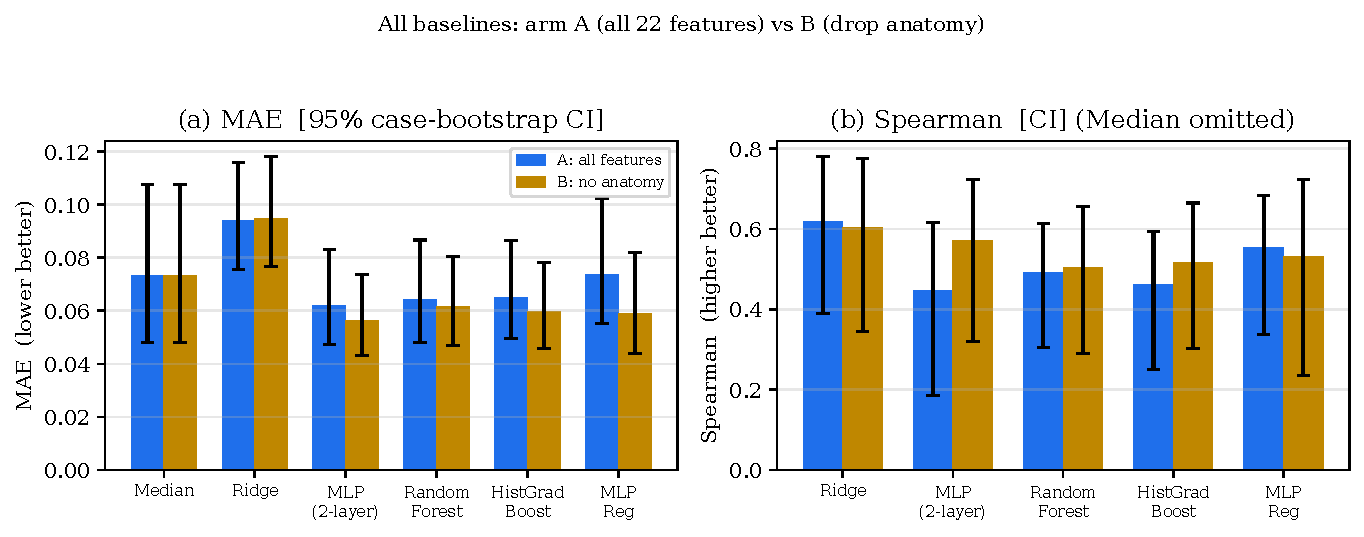
\includegraphics[width=\columnwidth]{figures/fig3_results.pdf}
\caption{All baselines, arm A (all features) vs B (no anatomy), with 95\%
case-bootstrap CI. The median floor is omitted from the Spearman panel (a constant
predictor has no ranking ability).}
\label{fig:bars}
\end{figure}

\begin{figure}[!t]
\centering
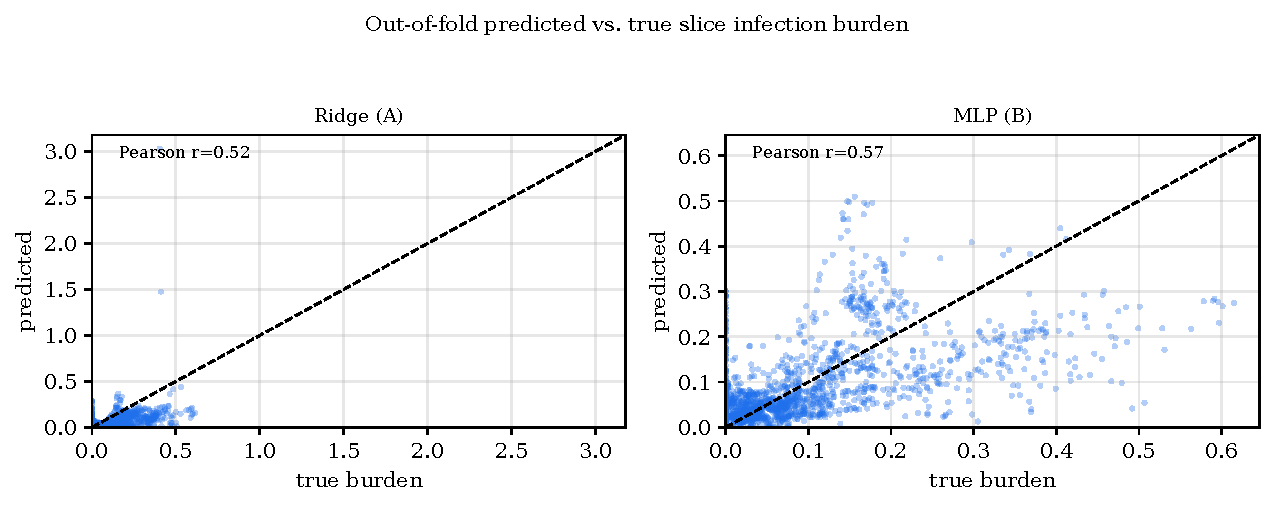
\includegraphics[width=\columnwidth]{figures/fig4_real_scatter.pdf}
\caption{Out-of-fold predicted vs.\ true slice infection burden (from
\texttt{data/real\_preds.npz}) for Ridge arm A and MLP arm B---the two best
MAE models. The dashed line is the identity; Pearson $r$ is shown per panel.}
\label{fig:scatter}
\end{figure}

\begin{figure}[!t]
\centering
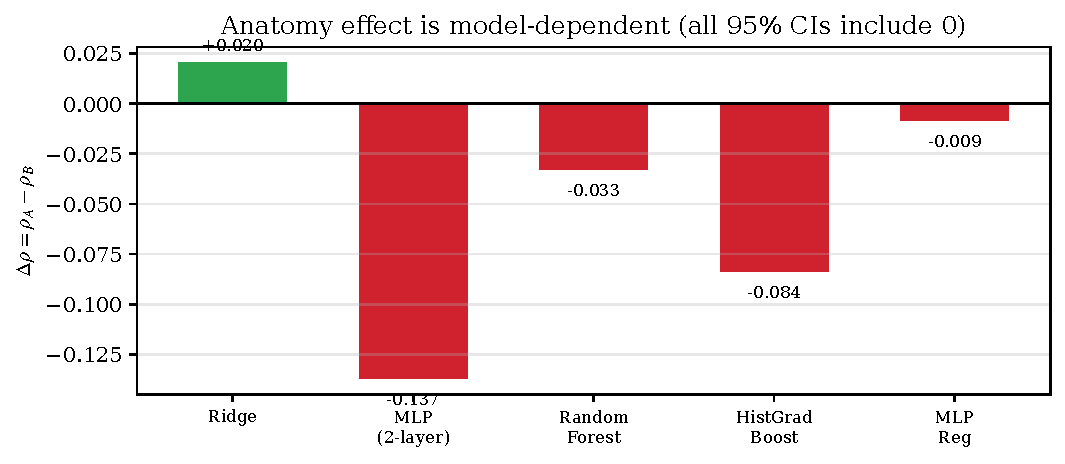
\includegraphics[width=\columnwidth]{figures/fig5_delta.pdf}
\caption{Anatomy effect $\Delta\rho=\rho_A-\rho_B$ per model family. The sign and
magnitude depend on the model: ridge and MLPRegressor gain a little from anatomy,
whereas the 2-layer MLP, Random Forest and HistGradient Boosting lose a little.
No bar clears its case-level CI, so the direction is model-dependent noise, not a
robust trend.}
\label{fig:delta}
\end{figure}

\section{Discussion}
We asked whether anatomical context helps slice-level infection-burden
regression. On this benchmark it does not, in any detectable sense, and the
case-level CIs make that statement quantitative rather than asserted. Three
reasons. \emph{(i)~Near-linear, low-dimensional anatomy.} The two anatomy
features are scalar and largely linear; a ridge model already exploits them, so
B costs it almost nothing, while nonlinear models can treat them as a shortcut
and overfit the 20 training cases. \emph{(ii)~Tiny effective sample.} Each test
fold holds $\sim5$ cases, so the Spearman CI half-width spans $\pm0.155$--$0.243$; no
A-vs-B difference clears it. \emph{(iii)~Mask-derived labels.} Where infection is
thin the mask is noisy, and the 28.2\% zero-infection slices dominate MAE and
mute any anatomy signal. Because $y$ is computed from masks rather than reader
scores, it measures \emph{mask} burden and inherits every segmentation error; we
make no clinical-severity claim.

\textbf{Why anatomy helps the linear model but not the MLP.} The direction of the
anatomy effect is itself model-dependent (Fig.~\ref{fig:delta}): ridge and
MLPRegressor gain a little from anatomy ($\Delta\rho{+}0.02$), whereas the
2-layer MLP, Random Forest and HistGradient Boosting lose a little. We can offer
three non-exclusive explanations but cannot disentangle them on 20 cases.
\emph{(a)~Collinearity.} The two anatomy features (lung-area ratio, left/right
ratio) are correlated with the lung-HU histogram and with each other; ridge's L2
shrinkage absorbs this shared, weak signal, while the unregularised MLP can treat
them as redundant and drop them. \emph{(b)~Capacity.} A 32-unit MLP has spare
capacity to fit the 1680 training slices through the other 20 features, so it
simply ignores anatomy; the linear ridge has no such slack and must use every
feature. \emph{(c)~Overfitting.} With only $15$ training cases per fold, the
MLP can absorb case-specific patterns through non-anatomy routes, and the anatomy
features---which vary mostly \emph{between} cases---add noise rather than
generalisable signal. Because every $\Delta\rho$ sits inside its case-level CI,
none of these mechanisms is confirmed here; we report the ambiguity rather than
assert a cause.

\textbf{Image-based learned baseline (ceiling).} We also trained a from-scratch
CNN on 32$\times$32 lung crops (conv 8$\times$3$\times$3, stride 2 $\to$ ReLU
$\to$ 2$\times$2 max-pool $\to$ linear, 250 epochs of batch GD). It collapsed to
predicting the training-mean burden and its OOF Spearman was non-positive, i.e.\
it did not learn on 20 cases; we therefore report the sanctioned downgrade,
Random-Conv-Features + Ridge (RCF). RCF reaches $\rho{=}0.558$---matching the
handcrafted-feature models---but its MAE $0.103$ is the highest of all, worse
than the median floor, because a fixed random-conv extractor captures \emph{rank}
order yet the ridge head mis-calibrates absolute burden. This suggests the 22-D
handcrafted features already extract most of the recoverable signal, and that a
learned pixel model needs far more than 20 cases to calibrate.

\textbf{Relation to clinical severity scoring.} Continuous, mask-derived burden is
the natural continuous analogue of ordinal scores such as RSNA or RALE, but it is
not a substitute for a reader's global assessment: masks ignore the texture
(ground-glass vs.\ consolidation) and distribution that radiologists weight, and a
slice-level label carries no sense of which lung region is involved. The benchmark
therefore establishes a \emph{reproducible floor} for automatic burden regression
and a clear negative result---anatomy does not help and a 20-case sample yields
wide CIs---rather than a clinically deployable score. We release it so that
stronger encoders and larger, multi-centre data can be measured against one fixed
partition.

\section{Reproducibility}
All artefacts are released so the benchmark is auditable. \emph{Dataset:}
COVID-19-CT-Seg (Ma et al.~\cite{ma2021covidseg}), Zenodo record 3757476,
\url{https://doi.org/10.5281/zenodo.3757476}, licensed CC-BY~4.0. \emph{Fixed
partition:} \texttt{data/splits.json} stores the seed-0 by-case 4-fold split, so
every result uses identical folds. \emph{Features:} \texttt{data/features.csv}
holds one row per slice (\texttt{case\_id}, \texttt{slice\_idx}, 22 features,
$y$). \emph{Code:} \texttt{src/train\_real\_v2.py} (regressors + CIs),
\texttt{src/cnn\_baseline.py} (image baseline),
\texttt{src/make\_figures\_real.py} (figures). \emph{Run:}
\texttt{python src/train\_real\_v2.py}; \texttt{python src/cnn\_baseline.py};
\texttt{python src/make\_figures\_real.py}---all seeds fixed (0).
\emph{Outputs:} \texttt{results/results\_real\_v2.json} (per-fold metrics, point
estimates, CIs), \texttt{data/real\_preds.npz} (out-of-fold predictions for
Fig.~\ref{fig:scatter}), and \texttt{BENCHMARK.md} (full protocol). Every script runs in minutes on a laptop
CPU; no GPU is required.

\section{Limitations}
\textbf{Sample size.} Twenty cases (2240 slices) is small; the effective unit is
the case, so every CI is wide and no A-vs-B difference is significant. This is a
benchmark and a sanity check, not an estimate of deployable accuracy.
\textbf{Slice-level labels from masks, not expert scores.} $y$ is computed from
segmentation masks, so it measures \emph{mask} burden and inherits every
segmentation error; it is not a radiologist reading and carries no clinical-
severity claim. \textbf{Single-centre public data.} All scans come from one
public release (COVID-19-CT-Seg) and may not represent other scanners, protocols
or populations, so the anatomy result may not transfer. Further, features are
hand-crafted (no learned encoder), regression is slice-wise with no 3-D
consistency, and we do not distinguish lesion types (GGO vs.\ consolidation).
Finally, with only 20 cases a leave-one-case-out scheme (20 test cases) would
use the data more efficiently than 4 folds; we leave it to future work.

\bibliographystyle{IEEEtran}
\bibliography{refs}

\end{document}
